% Final Year Project Report - SMART SUPPORT AI
% Meryem Nour Ben Abd Rahmen

\documentclass[12pt,a4paper]{report}

\usepackage[utf8]{inputenc}
\usepackage[T1]{fontenc}
\usepackage[english]{babel}
\usepackage[top=2.5cm,bottom=2.5cm,left=2.5cm,right=2.5cm]{geometry}
\usepackage{graphicx}
\usepackage[colorlinks=true,linkcolor=blue,urlcolor=blue,citecolor=blue]{hyperref}
\usepackage{fancyhdr}
\usepackage{setspace}
\usepackage{titlesec}
\usepackage{longtable}
\usepackage{booktabs}
\usepackage{float}
\usepackage{xcolor}
\usepackage{tikz}
\usepackage{pgf-umlcd}
\usetikzlibrary{arrows.meta,positioning,shapes.geometric,shapes.symbols,shapes.multipart}

\onehalfspacing
\setlength{\parindent}{1.5em}

% Headers and footers
\pagestyle{fancy}
\fancyhf{}
\fancyhead[L]{\small\textit{SMART SUPPORT AI}}
\fancyhead[R]{\small\leftmark}
\fancyfoot[C]{\thepage}
\renewcommand{\headrulewidth}{0.4pt}

\titleformat{\chapter}[display]{\normalfont\huge\bfseries}{\chaptertitlename\ \thechapter}{20pt}{\Huge}
\titlespacing*{\chapter}{0pt}{-20pt}{40pt}

\begin{document}

%=============================================================================
% TITLE PAGE
%=============================================================================
\begin{titlepage}
  \centering
  \vspace*{1.5cm}
  {\Large\textbf{University}}\\[0.5cm]
  {\large Faculty of Science}\\[0.3cm]
  {\large Department of Computer Science}\\[2cm]
  \vfill
  {\LARGE\textbf{Final Year Project Report}}\\[1cm]
  {\Huge\textbf{SMART SUPPORT AI}}\\[0.5cm]
  {\Large\textbf{Intelligent Customer Support}}\\[0.3cm]
  {\large Chatbot Application}\\[2cm]
  \vfill
  \begin{tabular}{ll}
    \textbf{Submitted by:} & Meryem Nour Ben Abd Rahmen \\[0.5cm]
    \textbf{Academic year:} & 2024--2025 \\[0.5cm]
    \textbf{Supervisor:} & \\[0.2cm]
    \textbf{Co-supervisor:} & \\[0.5cm]
  \end{tabular}
  \vfill
  {\large \today}
\end{titlepage}

%=============================================================================
% ACKNOWLEDGEMENTS
%=============================================================================
\chapter*{Acknowledgements}
\addcontentsline{toc}{chapter}{Acknowledgements}

I would like to express my sincere gratitude to all those who contributed to the completion of this final year project.

First and foremost, I thank my supervisor for his or her valuable guidance, sound advice, and availability throughout this work. His or her expertise and rigour have greatly shaped the quality of this report and of the application developed.

I also thank the teaching staff of the Department of Computer Science for the solid education provided during the degree programme, which enabled me to acquire the skills necessary for the design and implementation of a complete software application.

Finally, I thank my family and loved ones for their unfailing support and encouragement during this demanding period. This project would not have been completed without their patience and understanding.

%=============================================================================
% ABSTRACT
%=============================================================================
\chapter*{Abstract}
\addcontentsline{toc}{chapter}{Abstract}

This report presents \textbf{SMART SUPPORT AI}, an intelligent customer support chatbot application designed as a multi-tenant SaaS platform. The current context of customer service shows growing demand for responsiveness and availability while limiting human costs. Companies, especially SMEs, struggle to deliver quality support without dedicated resources.

The proposed solution is a platform that allows each company to create and customise its own chatbot, deploy it on its website or in a mobile application, and analyse its performance through an admin dashboard. The architecture relies on a Flutter mobile application for the management interface and user experience, a Supabase backend (PostgreSQL, authentication, functions) for persistence and business logic, and an intent-detection engine based on keywords and phrase similarity. An auto-learning system identifies recurring unanswered questions and allows the administrator to turn them into new intents, thus continuously improving the chatbot.

The project objectives are: to deliver an operational and scalable SaaS solution; to guarantee data isolation per company; to offer a modern user experience (chat, typing indicators, FAQ buttons); to integrate a handoff mechanism to human agents after repeated failures; and to provide partial offline mode (FAQ cache and deferred synchronisation). The methodology adopted follows an iterative approach: requirements analysis, design (actors, architecture, database), incremental implementation (auth, company, chat, admin, analytics, settings), and testing and validation.

The report details the study of existing solutions (human support, static FAQs, classical chatbots), analysis and design (actors, SaaS architecture, database schema, modules), technical implementation (Flutter, Supabase, chatbot logic, auto-learning, dashboard, integration, offline mode), as well as the testing strategy and results obtained. The conclusion highlights the contributions of the project and outlines future directions (neural AI, web widget, public API, advanced analytics).

\textbf{Keywords:} Chatbot, customer support, SaaS, multi-tenant, Flutter, Supabase, intent detection, auto-learning.

%=============================================================================
% TABLE OF CONTENTS
%=============================================================================
\tableofcontents

%=============================================================================
% CHAPTER 1 - GENERAL INTRODUCTION
%=============================================================================
\chapter{General Introduction}

\section{Context}

Customer support is a cornerstone of the relationship between companies and their users. With the growing digitalisation of services, customer expectations in terms of responsiveness, availability, and quality of answers have steadily increased. Traditional channels---telephone, email---remain essential but prove costly and difficult to scale for small and medium-sized enterprises (SMEs). At the same time, the rise of conversational assistants and chatbots has opened the way to partial or full automation of first-line support, making it possible to handle a large volume of repetitive requests while routing complex cases to human agents.

In this landscape, existing solutions range from expensive proprietary tools and poorly customisable ``black box'' chatbots to static FAQs that are often unengaging. There is strong demand from SMEs and start-ups for an affordable, customisable, and easily integrable solution that allows each organisation to deploy its own conversational assistant without advanced skills in artificial intelligence.

\section{Problem Statement}

The central problem of this project can be stated as follows: \textit{How to design and implement an intelligent customer support application, delivered as a service (SaaS), enabling multiple companies to create, configure, and deploy their own chatbot while ensuring data isolation, a quality user experience, and continuous improvement of answers through the analysis of unresolved questions?}

This problem encompasses several challenges: designing a secure and performant multi-tenant architecture; implementing a natural language understanding engine robust enough for production use (intent detection, keyword fallback); ensuring good ergonomics of the chat interface and the administration dashboard; and enabling the system to learn from failures by proposing new intents from recurring unanswered questions.

\section{Proposed Solution}

The proposed solution, \textbf{SMART SUPPORT AI}, is a SaaS platform that gives each company (tenant) its own space: account and company creation, brand configuration (colour, welcome message), intent management (training phrases and associated responses), analytics (sessions, messages, satisfaction, unanswered questions), and human handoff settings (email, WhatsApp). End users interact with the chatbot through a modern chat interface (message bubbles, typing indicator, quick FAQ buttons); after a configurable number of consecutive failures, the system offers handoff to a human via direct links (email, WhatsApp). An auto-learning mechanism allows the administrator to view the most frequently asked unanswered questions and turn them into new intents in one click.

The technical architecture is based on a Flutter mobile application (Clean Architecture, Riverpod, Material Design~3) for authentication, chat, administration, and settings screens, and on Supabase as the backend (PostgreSQL, authentication, and optionally Edge Functions). The chatbot logic (intent detection, recording of unknown questions, handoff triggering) is implemented on the client and/or server according to design choices, with the possibility of local FAQ caching for partial offline use.

\section{Objectives}

The project objectives are as follows:

\begin{enumerate}
  \item \textbf{Main objective:} Deliver an operational SaaS application that allows a company to create, configure, and use a personalised customer support chatbot, with strict data isolation per tenant.
  \item \textbf{Functional objectives:} Account and company management; authentication and role-based access (admin); creation and modification of intents (training phrases, responses); real-time conversation with intent detection and keyword fallback; recording of unanswered questions and suggestion of intent creation; dashboard (sessions, messages, satisfaction, average duration, pending questions); handoff configuration (email, WhatsApp); chatbot integration (web snippet, Flutter SDK, REST endpoint).
  \item \textbf{Technical objectives:} Clean and maintainable architecture (Flutter, Riverpod, separation of services/repositories); scalable backend (Supabase, PostgreSQL, RLS); polished user experience (Material~3, animations, partial offline mode).
\end{enumerate}

\section{Methodology}

The methodology adopted is iterative and delivery-oriented. An analysis phase formalised the requirements (actors, use cases, constraints) and studied the state of the art (human support, FAQs, chatbots). The design phase defined the overall architecture (multi-tenant SaaS), the database schema (companies, users, intents, chat\_sessions, messages, unknown\_questions, ratings), and the decomposition into modules (auth, company, chat, admin, analytics, settings). Implementation was carried out incrementally: core (auth, company, routing), chat engine and intent logic, Supabase persistence, dashboard and intent management, analytics, settings and integration. Testing (unit, integration, manual) accompanied each increment. Report writing was done in parallel and finalised after validation of the last scenarios.

%=============================================================================
% CHAPTER 2 - STATE OF THE ART
%=============================================================================
\chapter{State of the Art}

\section{Human Support}

Traditional customer support relies on teams of human agents reachable by phone, email, or live chat. This approach offers great flexibility and the ability to handle complex or emotional situations. However, it is costly, limited in availability (opening hours, response times), and difficult to scale with demand. SMEs often struggle to maintain a consistent level of service without outsourcing, which can damage the brand image. Human support remains indispensable for cases that exceed the capabilities of chatbots (complaints, disputes, highly specific requests).

\section{Static FAQ}

Frequently Asked Questions (FAQ) pages are a simple form of automation: answers are predefined and organised by topic. The user must browse the list or use a text search. The advantages are ease of implementation and no operational cost. The limitations are significant: no natural dialogue, no adaptation to the context of the question, no conversation tracking, and an often unengaging experience. Static FAQs usefully complement a chatbot but are not sufficient to offer an ``intelligent'' support experience.

\section{Classical Chatbots}

``Classical'' chatbots (rule-based or script-based) allow limited natural language interaction: keyword recognition, decision trees, or conditional response scripts. They are predictable and explainable, which facilitates maintenance and compliance with business processes. However, they struggle to handle the variety of formulations and off-script requests, often leading to generic answers or systematic transfers to humans. Chatbots based on deep learning (GPT-, BERT-type models, etc.) offer richer understanding but require computing resources and training data, and raise issues of cost, confidentiality, and control of responses. For a final year project and an SME audience, a hybrid approach---rules plus phrase similarity plus keyword fallback---constitutes a realistic and maintainable compromise.

\section{Comparative Analysis}

A comparative analysis of market solutions (Zendesk, Intercom, Dialogflow, open-source solutions such as Rasa) shows that generalist platforms often include a chatbot module but with pricing models and steep learning curves. Purely ``no-code'' solutions limit fine-grained customisation. Open-source frameworks offer great freedom but require ML/NLP expertise and dedicated infrastructure. A niche therefore exists for an SME-oriented SaaS solution: rapid deployment, intent customisation without AI skills, integrated dashboard, and controlled cost through a modern stack (Flutter, Supabase).

\section{Existing Limitations}

The limitations of existing solutions can be summarised as follows: prohibitive cost for small organisations; complexity of configuring advanced chatbots; lack of transparency on response logic; absence or insufficiency of self-improvement mechanisms from failures; and difficulty of integration into existing applications or sites without heavy development. The SMART SUPPORT AI project aims to address these limitations by offering a unified platform that is easy to adopt, with an explainable intent-detection engine and an auto-learning flow integrated into the dashboard.

%=============================================================================
% CHAPTER 3 - ANALYSIS AND DESIGN
%=============================================================================
\chapter{Analysis and Design}

\section{System Overview}

The SMART SUPPORT AI system is a SaaS platform that allows multiple companies (tenants) to create and manage their own customer support chatbot. Each company has an isolated space: brand settings, intents (training phrases and responses), chat sessions, unanswered questions, and ratings. End users interact with the chatbot via a chat interface; administrators access the dashboard to configure intents, view analytics, and manage settings (handoff, integration). The system records questions that the chatbot could not answer and aggregates them by frequency, allowing the admin to create new intents in one click (auto-learning).

\section{Actors}

The identified actors are as follows:

\begin{itemize}
  \item \textbf{Unauthenticated user:} views login and registration screens; may register (email, password) and then be redirected to company creation.
  \item \textbf{Administrator (authenticated):} belongs to a company; accesses chat, dashboard (intents, analytics, pending questions), settings (brand, handoff, integration), and logout.
  \item \textbf{System (chatbot):} receives user messages, queries the company's intents, detects the matching intent (or none), returns the response or records the question as unknown and optionally triggers handoff after N failures.
\end{itemize}

The ``agent'' role may be extended later (moderation, read-only access, etc.); in the current version, the ``admin'' role is sufficient for all management actions.

\section{Overall Architecture}

The overall architecture is client--server. The client is a Flutter mobile application (iOS, Android, and optionally Web) that handles the user interface, navigation (GoRouter), state (Riverpod), and backend calls. The server consists of Supabase services: PostgreSQL database, authentication (GoTrue), storage (files), and optionally Edge Functions for centralised business logic. Communication is via the Supabase REST API (with the Flutter SDK \texttt{supabase\_flutter}). Authentication is JWT-based; each request is associated with a user whose profile (table \texttt{users}) contains \texttt{company\_id}, allowing RLS (Row Level Security) policies to restrict access to that company's data.

\section{Multi-Tenant SaaS Architecture}

Multi-tenancy is ensured by the \texttt{company\_id} key present in all business tables (users, intents, chat\_sessions, messages, unknown\_questions, ratings). RLS policies on PostgreSQL filter rows according to the logged-in user's \texttt{company\_id} (obtained via the \texttt{users} table). Thus, company A can never access the intents, sessions, or messages of company B. The \texttt{companies} and \texttt{users} tables manage company creation (when the first admin registers) and the user--company--role association. Isolation is therefore logical (same schema, filtering by \texttt{company\_id}) and not physical (one database per client), which simplifies operations and updates.

\section{Database Modelling}

The database schema comprises the following entities:

\begin{itemize}
  \item \textbf{companies:} id (UUID), name, logo\_url, primary\_color, welcome\_message, support\_email, support\_whatsapp, subscription\_plan, created\_at.
  \item \textbf{users:} id (UUID, foreign key to auth.users), company\_id, role (admin, agent), email, created\_at.
  \item \textbf{intents:} id, company\_id, intent\_name, training\_phrases (JSONB), response\_text, created\_at.
  \item \textbf{chat\_sessions:} id, company\_id, user\_identifier, started\_at, end\_time, created\_at.
  \item \textbf{messages:} id, session\_id, sender (user \textbar\ bot), message, created\_at.
  \item \textbf{unknown\_questions:} id, company\_id, question, frequency, status (pending \textbar\ approved \textbar\ rejected), created\_at, updated\_at.
  \item \textbf{ratings:} id, session\_id, rating (1--5), feedback, created\_at.
\end{itemize}

A function \texttt{upsert\_unknown\_question(company\_id, question)} inserts a new unknown question or increments the \texttt{frequency} counter if the question already exists (case-insensitive comparison). Indexes on \texttt{company\_id}, \texttt{session\_id}, and \texttt{status} optimise dashboard and chat queries.

\section{Module Description}

\begin{enumerate}
  \item \textbf{Auth module:} Registration (email/password), login, logout; creation of \texttt{users} profile and \texttt{companies} company on first registration; loading of current profile and company (Riverpod providers).
  \item \textbf{Company module:} Read and update of company information (name, colour, welcome message, support email and WhatsApp); application of theme (primary colour) to the interface.
  \item \textbf{Chat module:} Session creation or retrieval; message sending; intent loading; intent detection (exact, contained, keywords); insertion of messages and unknown questions; handoff message triggering after N failures; display of bubbles, typing indicator, FAQ buttons, WhatsApp/Email buttons on handoff.
  \item \textbf{Admin module:} Dashboard (statistic cards: sessions, messages, satisfaction, average duration, pending questions, most asked); intent management screen (list, create, edit, delete); ``Suggestions'' tab (unknown questions with ``Create intent'' button).
  \item \textbf{Analytics module:} Aggregation of metrics (number of sessions, messages, average rating, average conversation duration, satisfaction rate, number of pending questions); list of most asked questions (from user messages).
  \item \textbf{Settings module:} Display of brand and handoff settings; copy of integration snippets (web widget, Flutter SDK, REST endpoint); logout.
  \item \textbf{Offline module:} Local cache of intents (SharedPreferences or equivalent); loading of intents from cache on network failure; offline message queue (structure ready for future synchronisation).
\end{enumerate}

%=============================================================================
% CHAPTER 4 - UML MODELING
%=============================================================================
\chapter{UML Modeling}

This chapter presents the main UML diagrams for the SMART SUPPORT AI system. The models describe the functional scope (use cases), the static structure (classes), the dynamic behaviour (sequence of interactions), the logical packaging (components), and the physical deployment of the application.

\section{Use Case Diagram}

The use case diagram captures the actors and the main functionalities they interact with. The Client User converses with the chatbot; the Company Admin manages intents, analytics, and company settings; the Support Agent may participate in human handoff when the bot escalates. Figure~\ref{fig:usecase} summarises these relationships within the system boundary.

\begin{figure}[H]
  \centering
  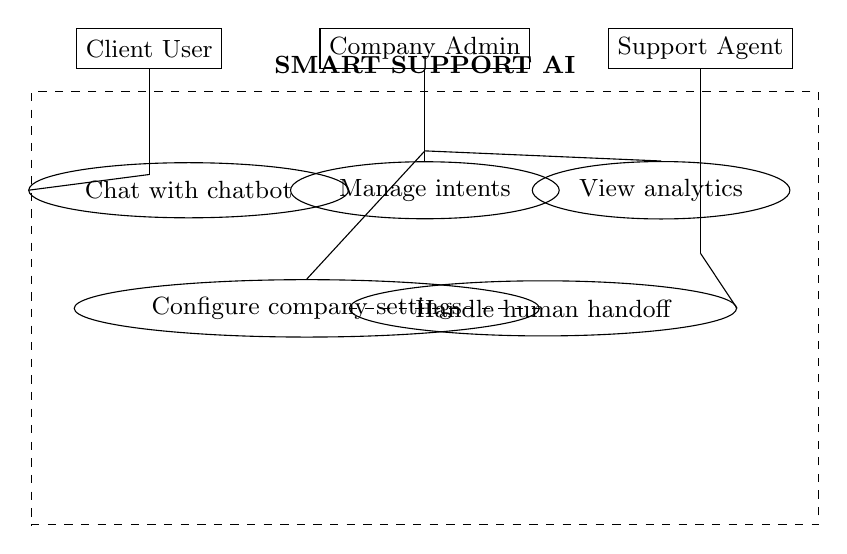
\begin{tikzpicture}[
    use case/.style={ellipse, draw=black, minimum width=1.8cm, minimum height=0.7cm, font=\small},
    actor/.style={rectangle, draw=black, minimum height=0.5cm, font=\small},
    sys/.style={rectangle, draw=black, dashed, minimum width=10cm, minimum height=5.5cm}
    ]
    \node[sys] (system) at (5,-2.5) {};
    \node[above=0.1cm of system.north, font=\small\bfseries] {SMART SUPPORT AI};

    \node[use case] (uc1) at (2,-1) {Chat with chatbot};
    \node[use case] (uc2) at (5,-1) {Manage intents};
    \node[use case] (uc3) at (8,-1) {View analytics};
    \node[use case] (uc4) at (3.5,-2.5) {Configure company settings};
    \node[use case] (uc5) at (6.5,-2.5) {Handle human handoff};

    \node[actor] (a1) at (1.5,0.8) {Client User};
    \draw[-] (a1.south) -- (1.5,-0.8);
    \draw[-] (1.5,-0.8) -- (uc1.west);

    \node[actor] (a2) at (5,0.8) {Company Admin};
    \draw[-] (a2.south) -- (5,-0.5);
    \draw[-] (5,-0.5) -- (uc2.north);
    \draw[-] (5,-0.5) -- (uc3.north);
    \draw[-] (5,-0.5) -- (uc4.north);

    \node[actor] (a3) at (8.5,0.8) {Support Agent};
    \draw[-] (a3.south) -- (8.5,-1.8);
    \draw[-] (8.5,-1.8) -- (uc5.east);

    \draw[-, dashed] (uc4.east) -- (uc5.west);
  \end{tikzpicture}
  \caption{Use case diagram: actors and main use cases.}
  \label{fig:usecase}
\end{figure}

\section{Class Diagram}

The class diagram reflects the core domain entities and their associations. Company and User are linked by company membership; ChatSession belongs to a Company and contains Messages; Intent and UnknownQuestion are scoped per Company; Rating is attached to a ChatSession. Figure~\ref{fig:class} illustrates this structure with key attributes.

\begin{figure}[H]
  \centering
  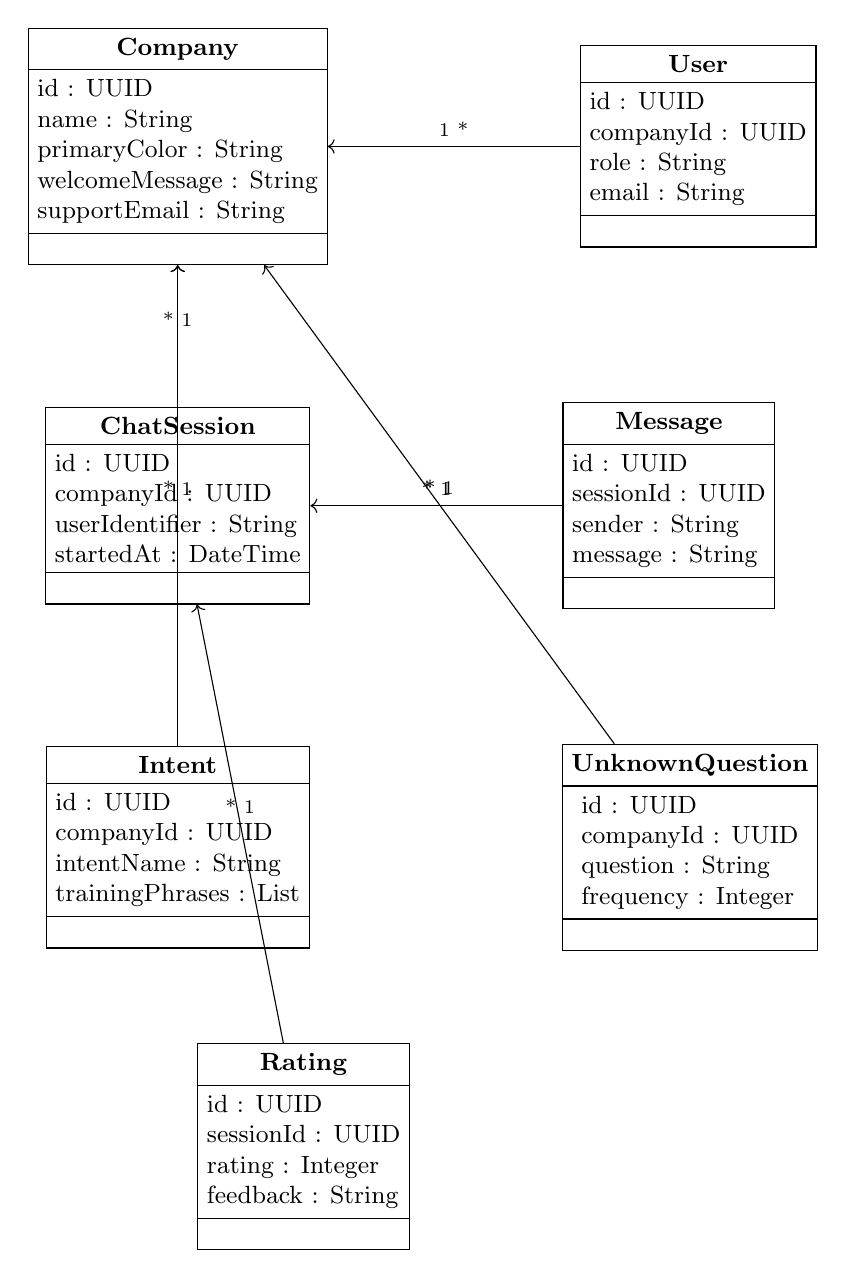
\begin{tikzpicture}[
    class/.style={rectangle split, rectangle split parts=3, draw=black, font=\small, align=left},
    node distance=0.2cm
    ]
    \node[class] (Company) at (0,0) {
      \textbf{Company}
      \nodepart{second}
      id : UUID \\
      name : String \\
      primaryColor : String \\
      welcomeMessage : String \\
      supportEmail : String
      \nodepart{third}
    };
    \node[class, right=3.2cm of Company] (User) {
      \textbf{User}
      \nodepart{second}
      id : UUID \\
      companyId : UUID \\
      role : String \\
      email : String
      \nodepart{third}
    };
    \node[class, below=1.8cm of Company] (ChatSession) {
      \textbf{ChatSession}
      \nodepart{second}
      id : UUID \\
      companyId : UUID \\
      userIdentifier : String \\
      startedAt : DateTime
      \nodepart{third}
    };
    \node[class, right=3.2cm of ChatSession] (Message) {
      \textbf{Message}
      \nodepart{second}
      id : UUID \\
      sessionId : UUID \\
      sender : String \\
      message : String
      \nodepart{third}
    };
    \node[class, below=1.8cm of ChatSession] (Intent) {
      \textbf{Intent}
      \nodepart{second}
      id : UUID \\
      companyId : UUID \\
      intentName : String \\
      trainingPhrases : List
      \nodepart{third}
    };
    \node[class, right=3.2cm of Intent] (UnknownQuestion) {
      \textbf{UnknownQuestion}
      \nodepart{second}
      id : UUID \\
      companyId : UUID \\
      question : String \\
      frequency : Integer
      \nodepart{third}
    };
    \node[class, below=1.2cm of Intent, xshift=1.6cm] (Rating) {
      \textbf{Rating}
      \nodepart{second}
      id : UUID \\
      sessionId : UUID \\
      rating : Integer \\
      feedback : String
      \nodepart{third}
    };
    \draw[->] (User) -- (Company) node[midway, above, font=\scriptsize] {1 *};
    \draw[->] (ChatSession) -- (Company) node[midway, above, font=\scriptsize] {* 1};
    \draw[->] (Message) -- (ChatSession) node[midway, above, font=\scriptsize] {* 1};
    \draw[->] (Intent) -- (Company) node[midway, above, font=\scriptsize] {* 1};
    \draw[->] (UnknownQuestion) -- (Company) node[midway, above, font=\scriptsize] {* 1};
    \draw[->] (Rating) -- (ChatSession) node[midway, above, font=\scriptsize] {* 1};
  \end{tikzpicture}
  \caption{Class diagram: domain entities and relationships.}
  \label{fig:class}
\end{figure}

\section{Sequence Diagram}

The sequence diagram in Figure~\ref{fig:seq} describes the flow when a user sends a message: the Flutter app calls the Chat Service, which creates or retrieves the session and stores the message via the Supabase API; the Chat Service loads intents, runs intent detection, and optionally saves an unknown question; the response is written to the database and returned to the app, which updates the UI.

\begin{figure}[H]
  \centering
  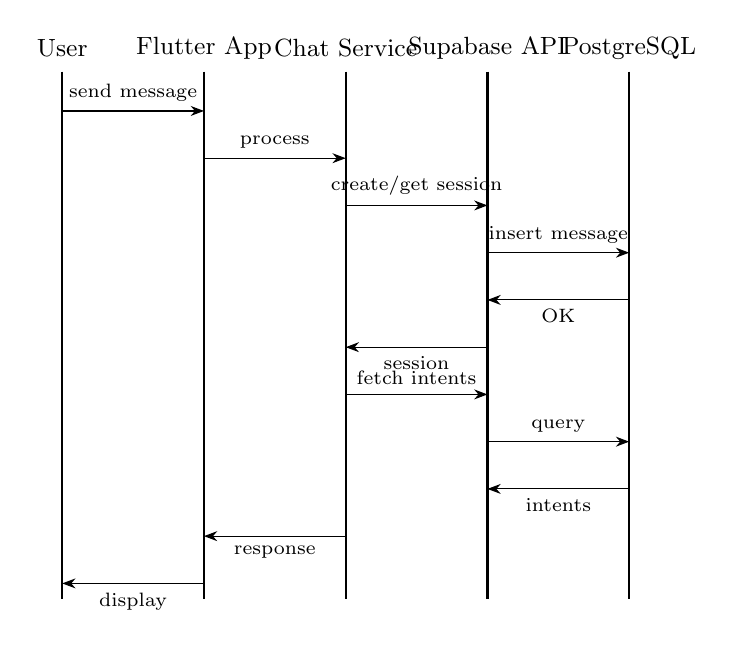
\begin{tikzpicture}[
    node distance=0.8cm,
    every node/.style={font=\small},
    lifeline/.style={draw=black, thick},
    msg/.style={->, >=Stealth, draw=black}
    ]
    \node (user) at (0,0) {User};
    \node (app) at (1.8,0) {Flutter App};
    \node (chat) at (3.6,0) {Chat Service};
    \node (api) at (5.4,0) {Supabase API};
    \node (db) at (7.2,0) {PostgreSQL};

    \draw[lifeline] (0,-0.3) -- (0,-7);
    \draw[lifeline] (1.8,-0.3) -- (1.8,-7);
    \draw[lifeline] (3.6,-0.3) -- (3.6,-7);
    \draw[lifeline] (5.4,-0.3) -- (5.4,-7);
    \draw[lifeline] (7.2,-0.3) -- (7.2,-7);

    \draw[msg] (0,-0.8) -- (1.8,-0.8) node[midway, above, font=\scriptsize] {send message};
    \draw[msg] (1.8,-1.4) -- (3.6,-1.4) node[midway, above, font=\scriptsize] {process};
    \draw[msg] (3.6,-2) -- (5.4,-2) node[midway, above, font=\scriptsize] {create/get session};
    \draw[msg] (5.4,-2.6) -- (7.2,-2.6) node[midway, above, font=\scriptsize] {insert message};
    \draw[msg] (7.2,-3.2) -- (5.4,-3.2) node[midway, below, font=\scriptsize] {OK};
    \draw[msg] (5.4,-3.8) -- (3.6,-3.8) node[midway, below, font=\scriptsize] {session};
    \draw[msg] (3.6,-4.4) -- (5.4,-4.4) node[midway, above, font=\scriptsize] {fetch intents};
    \draw[msg] (5.4,-5) -- (7.2,-5) node[midway, above, font=\scriptsize] {query};
    \draw[msg] (7.2,-5.6) -- (5.4,-5.6) node[midway, below, font=\scriptsize] {intents};
    \draw[msg] (3.6,-6.2) -- (1.8,-6.2) node[midway, below, font=\scriptsize] {response};
    \draw[msg] (1.8,-6.8) -- (0,-6.8) node[midway, below, font=\scriptsize] {display};
  \end{tikzpicture}
  \caption{Sequence diagram: user sends message, flow through Chat Service and Supabase to response.}
  \label{fig:seq}
\end{figure}

\section{Component Diagram}

The component diagram (Figure~\ref{fig:comp}) shows the main logical blocks: the Flutter Mobile App (UI and client logic), the Chatbot Engine (intent detection and response logic), the Supabase API (auth and data access), the PostgreSQL Database (persistence), and the Admin Dashboard (part of the Flutter app, consuming analytics and settings). Dependencies between components are indicated by the provided/required interfaces and connections.

\begin{figure}[H]
  \centering
  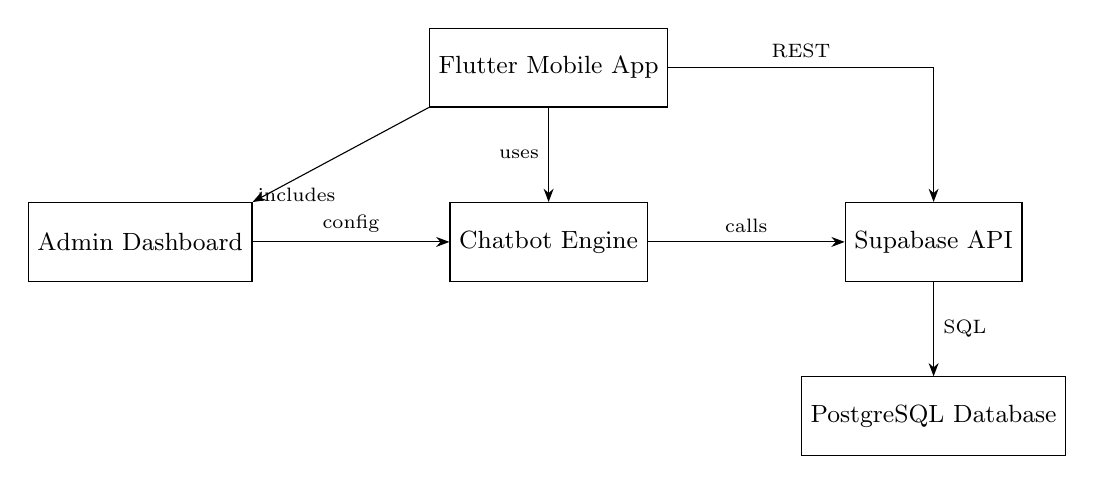
\begin{tikzpicture}[
    comp/.style={rectangle, draw=black, minimum width=2.2cm, minimum height=1cm, font=\small},
    node distance=1.2cm
    ]
    \node[comp] (flutter) {Flutter Mobile App};
    \node[comp, below=of flutter] (engine) {Chatbot Engine};
    \node[comp, right=2.5cm of engine] (api) {Supabase API};
    \node[comp, below=of api] (db) {PostgreSQL Database};
    \node[comp, left=2.5cm of engine] (admin) {Admin Dashboard};

    \draw[->, >=Stealth] (flutter.south) -- (engine.north) node[midway, left, font=\scriptsize] {uses};
    \draw[->, >=Stealth] (flutter.east) -| (api.north) node[near start, above, font=\scriptsize] {REST};
    \draw[->, >=Stealth] (engine.east) -- (api.west) node[midway, above, font=\scriptsize] {calls};
    \draw[->, >=Stealth] (api.south) -- (db.north) node[midway, right, font=\scriptsize] {SQL};
    \draw[->, >=Stealth] (flutter.south west) -- (admin.north east) node[near end, below, font=\scriptsize] {includes};
    \draw[->, >=Stealth] (admin.east) -- (engine.west) node[midway, above, font=\scriptsize] {config};
  \end{tikzpicture}
  \caption{Component diagram: main system components and their dependencies.}
  \label{fig:comp}
\end{figure}

\section{Deployment Diagram}

The deployment diagram (Figure~\ref{fig:deploy}) describes the physical distribution: the Mobile Device runs the Flutter application; a Web Browser may host a future web widget; both communicate over an Internet Connection with the Supabase Cloud node, which hosts the API and the PostgreSQL database. This reflects the SaaS delivery model and the separation between client devices and the centralised backend.

\begin{figure}[H]
  \centering
  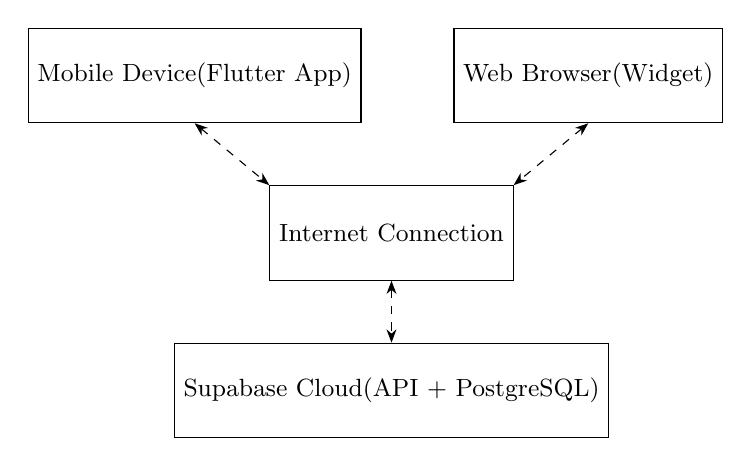
\begin{tikzpicture}[
    node/.style={rectangle, draw=black, minimum width=2.5cm, minimum height=1.2cm, font=\small},
    conn/.style={draw=black, dashed, <->, >=Stealth}
    ]
    \node[node] (mobile) at (0,0) {Mobile Device \\ (Flutter App)};
    \node[node] (browser) at (5,0) {Web Browser \\ (Widget)};
    \node[node] (internet) at (2.5,-2) {Internet Connection};
    \node[node] (cloud) at (2.5,-4) {Supabase Cloud \\ (API + PostgreSQL)};

    \draw[conn] (mobile.south) -- (internet.north west);
    \draw[conn] (browser.south) -- (internet.north east);
    \draw[conn] (internet.south) -- (cloud.north);
  \end{tikzpicture}
  \caption{Deployment diagram: nodes and communication paths.}
  \label{fig:deploy}
\end{figure}

%=============================================================================
% CHAPTER 5 - IMPLEMENTATION
%=============================================================================
\chapter{Implementation}

\section{Technical Environment}

The development environment includes: Flutter (stable SDK, stable channel) for the mobile application; Dart 3.x; editor/IDE (VS Code or Android Studio) with Flutter and Dart extensions; Supabase (cloud account or self-hosted instance) for the PostgreSQL database, authentication, and API; Git for version control. Flutter packages used include \texttt{flutter\_riverpod}, \texttt{supabase\_flutter}, \texttt{go\_router}, \texttt{google\_fonts}, \texttt{url\_launcher}, \texttt{shared\_preferences}, \texttt{connectivity\_plus}, and \texttt{cached\_network\_image}. Build and testing are done with \texttt{flutter pub get}, \texttt{flutter analyze}, and \texttt{flutter test}.

\section{Software Architecture}

The Flutter application's software architecture follows a layered organisation inspired by Clean Architecture: \texttt{core} (constants, theme, router), \texttt{models} (business entities: Company, AppUser, ChatIntent, ChatSession, ChatMessage, UnknownQuestion, SessionRating), \texttt{services} (SupabaseService, AuthService, IntentService, ChatApiService, ChatLogicService, AnalyticsService, UnknownQuestionsService, OfflineCacheService), \texttt{repositories} (CompanyRepository, IntentRepository, ChatRepository), and \texttt{features} (auth, company, chat, admin, analytics, settings, splash). Each feature contains screens (presentation/screens) and Riverpod providers (presentation/providers). State management is centralised via Riverpod (FutureProvider for asynchronous data, StateProvider for local chat state). The GoRouter handles named routes (splash, login, register, company-setup, chat, admin, analytics, intents, settings).

\section{Flutter Application}

The Flutter application is structured around main screens: \textbf{SplashScreen} (redirect to chat if valid session, otherwise login); \textbf{LoginScreen} and \textbf{RegisterScreen} (email/password forms, Supabase Auth calls); \textbf{CompanySetupScreen} (company and user profile creation after first registration); \textbf{ChatScreen} (message list, input field, FAQ buttons, user/bot bubbles, typing indicator, handoff buttons); \textbf{AdminDashboardScreen} (action grid and statistic cards, ``most asked questions'' section); \textbf{IntentManagementScreen} (Intents and Suggestions tabs, intent creation dialog, intent creation from a suggestion); \textbf{AnalyticsScreen} (detailed list of metrics); \textbf{SettingsScreen} (settings display, integration dialog, logout). The theme (Material Design~3) is applied globally; the primary colour can be overridden dynamically from \texttt{company.primary\_color} to reflect the company brand.

\section{Supabase Backend}

The Supabase backend provides: a PostgreSQL database with the tables and the \texttt{upsert\_unknown\_question} function described in Chapter~3; email/password authentication (GoTrue); RLS policies to restrict row access by \texttt{company\_id}; and the auto-generated REST API. The schema is deployed via a migration file (e.g.\ \texttt{supabase/migrations/20250228000000\_initial\_schema.sql}). Keys (project URL and anon key) are configured in the application via environment variables or \texttt{--dart-define} so as not to expose them in source code.

\section{Chatbot Operation}

The chatbot flow is as follows: (1) the user sends a message; (2) the client creates or retrieves the session (\texttt{chat\_sessions}) and inserts the message (\texttt{messages}, sender = user); (3) the company's intents are loaded (from Supabase or from the offline cache); (4) the \texttt{ChatLogicService} compares the message to the list of training phrases: first exact match (after normalisation), then match by inclusion (longest phrase first), then keyword overlap score (minimum threshold of 2 words); (5) if an intent is found, the associated response is returned and the failure counter is reset; (6) otherwise, the question is recorded via \texttt{upsert\_unknown\_question}, the failure counter is incremented, and if the counter reaches 2 (configurable), a handoff message is returned (with email/WhatsApp links if configured), otherwise a generic message (``I couldn't find an answer, could you rephrase?''); (7) the bot's response is inserted into \texttt{messages} and the displayed message list is updated.

\section{Auto-Learning System}

The auto-learning system relies on the \texttt{unknown\_questions} table and the ``Suggestions'' screen of the Admin module. Whenever a question matches no intent, it is recorded (or its \texttt{frequency} counter incremented). The administrator consults the list of questions in ``pending'' status, sorted by frequency. For each question, he or she can: (a) click ``Create intent from this suggestion'': a dialog opens with the intent name and training phrases pre-filled (the suggested question), and a field for the response; after creation, the intent is added and the question is marked ``approved''; (b) mark the question as approved without creating an intent; (c) delete or reject the question. Thus, recurring uncovered formulations quickly become new intents, improving the resolution rate without heavy manual intervention.

\section{Analytics Dashboard}

The admin dashboard displays: total number of sessions and messages; satisfaction rate (proportion of ratings $\geq 4$ out of all ratings); percentage of unanswered questions (indicator derived from \texttt{unknown\_questions} and sessions); average conversation duration (difference between \texttt{end\_time} and \texttt{started\_at} for completed sessions); number of pending questions (``pending'' status); and a ``most asked questions'' section based on aggregation of user messages by text (top 5 or 10). Data is retrieved via \texttt{AnalyticsService}, which runs Supabase queries (with joins and \texttt{company\_id} filters) and returns cards and lists formatted for the interface.

\section{Chatbot Integration}

Integration of the chatbot into third-party systems is documented and exposed in the Settings screen: (1) \textbf{Web widget:} an HTML snippet to insert before \texttt{</body>} loads an external script with \texttt{data-company-id}; (2) \textbf{Flutter SDK:} a \texttt{SmartSupportChatWidget} component (or equivalent) can be embedded in another Flutter application by passing \texttt{companyId} and optional parameters; (3) \textbf{REST endpoint:} an example \texttt{POST /v1/chat} request with \texttt{company\_id} and \texttt{message} is provided for custom clients. Full implementation of the web widget and REST API can form a project extension (Edge Function or dedicated server).

\section{Offline Mode}

Partial offline mode is provided by \texttt{OfflineCacheService}: after each successful load of intents from Supabase, the list is serialised (JSON) and stored locally (SharedPreferences) with a key depending on \texttt{company\_id}. On network failure when loading intents, the service attempts to return cached intents; if the cache is empty, the error is propagated. An offline message queue structure (list of messages not yet sent) is in place for future synchronisation when connectivity returns; the interface can be extended to show an ``offline'' indicator and disable sending or queue messages.

%=============================================================================
% CHAPTER 5 - TESTING AND VALIDATION
%=============================================================================
\chapter{Testing and Validation}

\section{Testing Strategy}

The testing strategy combines unit tests (isolated business logic), integration tests (providers, services with mocks), and manual tests (full flows on emulator or device). Unit tests focus primarily on \texttt{ChatLogicService} (normalisation, exact match, by inclusion, by keywords) and on models (JSON deserialisation). Integration tests verify that Riverpod providers (currentUserProvider, currentCompanyProvider, intentsProvider) update correctly after simulated operations. Manual tests cover: registration, login, company creation, intent addition, message sending (with and without match), handoff triggering, dashboard and suggestions consultation, intent creation from a suggestion, and logout. Tests with Supabase in the development environment use a test project to avoid altering production data.

\section{Test Cases}

Representative test cases include: (1) \textbf{Registration and company creation:} a new user registers with email and password; after redirect to CompanySetupScreen, he or she enters the company name and welcome message; the company and user profile are created in the database; redirect to ChatScreen occurs. (2) \textbf{Intent detection:} an intent ``Opening hours'' with phrases ``What are the opening hours?'' and ``Hours of operation'' and response ``We are open Monday to Friday, 9am--6pm.''; the user sends ``What are the opening hours?''; the bot replies with the configured response. (3) \textbf{Unanswered question and handoff:} the user sends two consecutive messages with no match; after the second, the handoff message is displayed with WhatsApp and Email buttons if configured. (4) \textbf{Auto-learning:} after several questions ``How do I cancel an order?'' with no intent, the question appears in the Suggestions tab with its frequency; the admin clicks ``Create intent'', fills in the response, and validates; the new intent is available and the question is marked approved. (5) \textbf{Offline:} after loading intents once, connectivity is cut; reloading intents uses the cache and the interface remains usable for already known intents.

\section{Results}

Manual tests on Android and iOS emulators confirmed the correct execution of the main flows: authentication, company creation, chat with intent detection and handoff, access to dashboard and analytics, intent and suggestion management. Tests of \texttt{ChatLogicService} (run via \texttt{flutter test}) validate exact, contained, and keyword match cases, as well as no-match cases. No critical blocking issues were observed; a few linter warnings (unnecessary casts, preference for \texttt{const}) were addressed or documented. Performance remains acceptable for a reasonable volume of messages and intents (a few hundred per company).

\section{Discussion}

Current limitations concern: purely lexical intent detection (no deep semantics), which may generate false positives or negatives on distant formulations; the absence of actual deployment of the web widget and REST API (documentation and structure are in place); and the fact that synchronisation of messages queued offline is not yet implemented. Validation nevertheless demonstrates that the main objective---delivering an operational SaaS application that allows a company to configure and use a chatbot with data isolation, handoff, and auto-learning---is achieved. Feedback could steer a V2 towards detection using a lightweight language model (embeddings + similarity) or deeper integration (hosted web widget, public API).

%=============================================================================
% GENERAL CONCLUSION
%=============================================================================
\chapter*{General Conclusion}
\addcontentsline{toc}{chapter}{General Conclusion}

This final year project has made it possible to design and implement \textbf{SMART SUPPORT AI}, an intelligent customer support chatbot application that can be deployed as a multi-tenant SaaS service. The set objectives have been met: a company can register, create its company, configure its intents (training phrases and responses), deploy a modern chat experience (bubbles, typing indicator, FAQ buttons), benefit from human handoff after repeated failures (email, WhatsApp), and continuously improve the bot through the analysis of unanswered questions and the creation of intents from suggestions. The technical architecture (Flutter, Supabase, PostgreSQL, RLS) ensures data isolation per tenant and a maintainable, evolutive base.

The project's contributions are both technical---mastery of a modern stack (Flutter, Riverpod, Supabase), design of an explainable intent-detection engine and an auto-learning flow integrated into the dashboard---and functional---an operational deliverable usable in real conditions for SMEs or demonstrations. The writing of this report has made it possible to structure and formalise the context, problem statement, state of the art, analysis and design, implementation, and validation, within an academic and professional framework.

\section*{Future Perspectives}

Several directions for evolution can be considered: (1) \textbf{Enrichment of the understanding engine:} integration of an embeddings model (sentence transformers) or a small BERT-type model for semantic similarity, while keeping the rule-based fallback for traceability; (2) \textbf{Web widget deployment:} development of a lightweight JavaScript script loaded by client sites, communicating with a dedicated API or a Supabase Edge Function; (3) \textbf{Public REST API:} exposure of a documented (OpenAPI) and secured (API keys per company) \texttt{POST /v1/chat} endpoint for third-party integrations; (4) \textbf{Advanced analytics:} charts of session and satisfaction evolution over time, CSV export, customisable dashboards; (5) \textbf{Roles and permissions:} extension of the model (read-only ``agent'' role, suggestion moderation) and fine-grained permission management in the interface. These perspectives would strengthen SMART SUPPORT AI's position as a complete and scalable solution for SME customer support.

%=============================================================================
% END OF DOCUMENT
%=============================================================================
\end{document}
